\section{Characteristics of feature vectors}
\label{section:real-characteristics}

This section contains the analysis and discussion on the properties of the data representations generated by various Deep Learning models –~and how these properties affect (or not) the performance of OOD detection methods. The results correspond to observations made in previous sections (e.g., table \ref{tab:image-auroc}, figures \ref{fig:image-auroc}, \ref{fig:text-auroc}, \ref{fig:image-classification} and \ref{fig:text-classification}).

The table \ref{tab:image-dimensions} summarizes the dimensionality of feature vectors for image data –~coming from the utilized representations models (CLIP, CoCa, ConvNeXT, EfficientNet, ResNet, ViT). The table \ref{tab:text-dimensions} covers analogous information regarding the feature vectors obtained for text documents from models (BERT, Doc2Vec, fastText, TF-IDF).

Figures \ref{fig:characteristics-image}, \ref{fig:characteristics-text-20newsgroups}, \ref{fig:characteristics-text-banking77} illustrate the various discovered properties of the feature vectors, per in-distribution data class and utilized representation model, obtained for the image data (ImageNet), long (20newsgroups) and short (banking77) text documents, respectively. The considered values are as follows:
\vspace{-0.5\baselineskip}
\begin{itemize}
    \item variance – calculated as an average value over all features in a given class,
    \item correlation – an average of the absolute values calculated within the top triangle of the covariance matrix,
    \item kurtosis – computed as an average over all features for each class; value $3.0$ corresponds to normal-like distribution, big values indicate long tails, low values are related to highly-concentrated data.
    \item skewness – also calculated as an average value over all features; values in range $(-0.5, 0.5)$ mean that distribution is approximately symmetric, for values $(0.5, 1.0)$ the distribution is slightly skewed and for values $(1.0; \infty)$ it is considered a~highly skewed distribution.
    \item test of normality – average $p$-value obtained for each feature in class, using the D’Agostino and Pearson’s test\footnote{\url{https://docs.scipy.org/doc/scipy/reference/generated/scipy.stats.normaltest.html}} with assumption of the Gaussian distribution as~the~null-hypothesis.
    \item number of feature-wise outliers – the average number of observations that fall outside the confidence interval (range $\pm1.5$ IQR threshold) based on the values of each feature in the training clusters vectors.
\end{itemize}

Important observation for all the analyzed cases is that, in general, there are no strongly correlated features – all medians of absolute correlations are below $0.25$. However the observed correlations vary per class, especially significantly for some representations (EfficientNet and BERT), and this raises the question of justification for utilization of the pooled covariance matrix. As classes present various correlations, the single covariance matrix incorrectly reflects data from some of these classes, i.e., it~results in an~important method error, visible as low performance of MDP measure.

The features produced by ResNet are especially weakly correlated, which corresponds with high efficiency of SED measure with this representation in conducted experiments. Contrary, EfficientNet is characterized by higher correlations, hence the MD performs better than SED in that case (i.e., ignoring the correlations leads to worse performance).

Similarly, there are no significant differences in average variances of features observed. Although the BERT, CoCa and fastText produced feature vectors of especially low average variance. Most representations produce features that appear symmetric (BERT, CLIP, CoCa, ConvNeXT, Doc2Vec, fastText and ViT), with exception of EfficientNet and ResNet, where the valued are highly skewed – and additionally, in case of ResNet, widely distributed with long tails.

For TF-IDF the SED measure was impossible to utilize due to multiple empty features in obtained vectors, i.e., zero-variance calculated and therefore division by zero encountered in formula \ref{eq:sed} (section \ref{section:SEuclidean}). Also, because of the TF-IDF feature vectors sizes, the estimation of properties such as correlations was time-consuming and hence it is omitted in the figures.

It must be noticed that the characteristics obtained for short and long text documents differ significantly in some cases, e.g., in the normality tests (figures \ref{fig:text-20newsgroups-pvalue} and \ref{fig:text-banking77-pvalue}). This corresponds with inconsistencies observed fpr results of AUROC, sensitivity and specificity scores between 20newsgroups and banking77, presented in previous sections. Hence, a more detailed study of the relation between the characteristics and the ID data shall be conducted in the future.

\begin{table}[t]
    \centering
    \small
    \setlength{\tabcolsep}{0.56em}
    \renewcommand{\arraystretch}{1.5}
    \begin{tabular}{l|ccccccc}
        \toprule
        \toprule
            representation
            & CLIP
            & CoCa
            & ConvNeXT
            & EfficientNet
            & MobileNet
            & ResNet
            & ViT
            \\
        \midrule
            dimension $d$
            & 1024
            & 769
            & 1536
            & 1280
            & 1280
            & 2048
            & 1024
            \\
        \bottomrule
        \bottomrule
    \end{tabular}
    \caption{Dimensionality of the feature vectors used for image representations.}
    \label{tab:image-dimensions}
    \vspace{-0.5em}  % spacing hack
    \begin{tabular}{l|cccccc}
        \toprule
        \toprule
            representation
            & BERT-base
            & BERT-tiny
            & Doc2Vec
            & fastText
            & ${}^\text{~~~~TF-IDF}_\text{\tiny(20newsgroups)}$
            & ${}^\text{~\,TF-IDF}_\text{\tiny(banking77)}$
            \\
        \midrule
            dimension $d$
            & 768
            & 128
            & 300
            & 100
            & 5000
            & 2095
            \\
        \bottomrule
        \bottomrule
    \end{tabular}
    \caption{Dimensionality of the feature vectors used for text representations.}
    \label{tab:text-dimensions}
    \vspace{-1.8em}  % spacing hack
\end{table}

\begin{figure}[t]
    % StreamLit settings: width=5, height=3
    \centering
    \begin{subfigure}[b]{0.495\textwidth}
        \centering
        \caption{\small Correlation of features}
        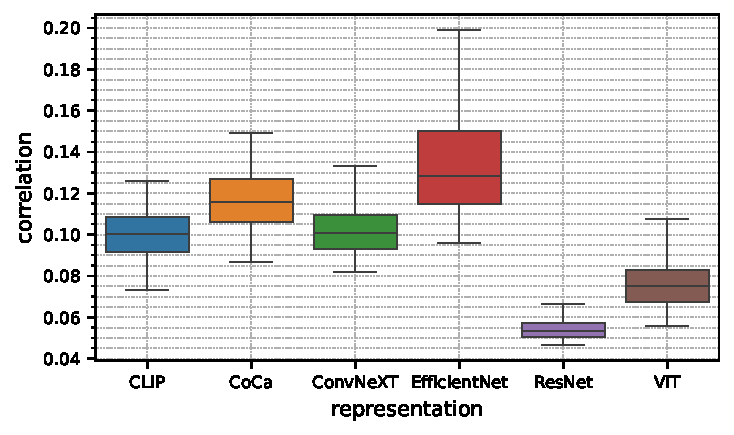
\includegraphics[width=\textwidth]{images/real-characteristics/image/properties-ImageNet-abscorr(representation,representation)-representation_CLIP,CoCa,ConvNeXT,EfficientNet,ResNet,ViT-class_0,999-data_ID-train.pdf}
        \label{fig:image-abscorr}
    \end{subfigure}
    \hfill
    \begin{subfigure}[b]{0.495\textwidth}
        \centering
        \caption{\small Variance of features}
        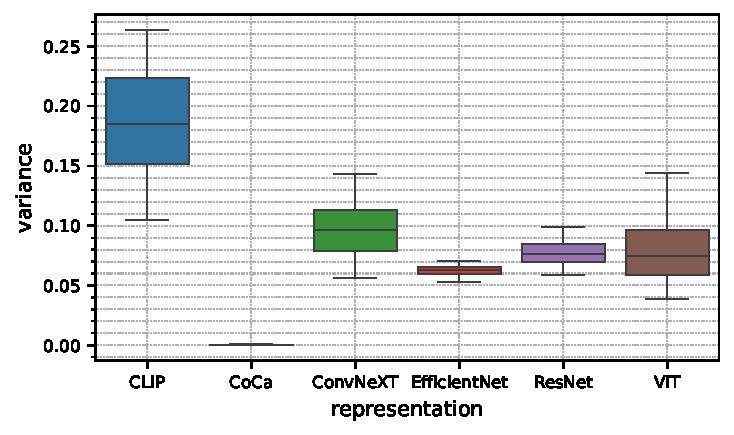
\includegraphics[width=\textwidth]{images/real-characteristics/image/properties-ImageNet-var(representation,representation)-representation_CLIP,CoCa,ConvNeXT,EfficientNet,ResNet,ViT-class_0,999-data_ID-train.pdf}
        \label{fig:image-var}
    \end{subfigure}
    \begin{subfigure}[b]{0.495\textwidth}
        \centering
        \caption{\small Number of outliers per feature}
        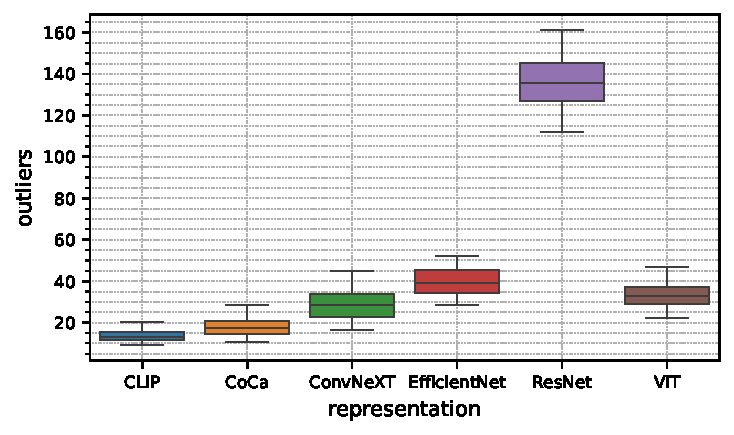
\includegraphics[width=\textwidth]{images/real-characteristics/image/properties-ImageNet-noutliers(representation,representation)-representation_CLIP,CoCa,ConvNeXT,EfficientNet,ResNet,ViT-class_0,999-data_ID-train.pdf}
        \label{fig:image-outliers}
    \end{subfigure}
    \hfill
    \begin{subfigure}[b]{0.495\textwidth}
        \centering
        \caption{\small Test of features normality}
        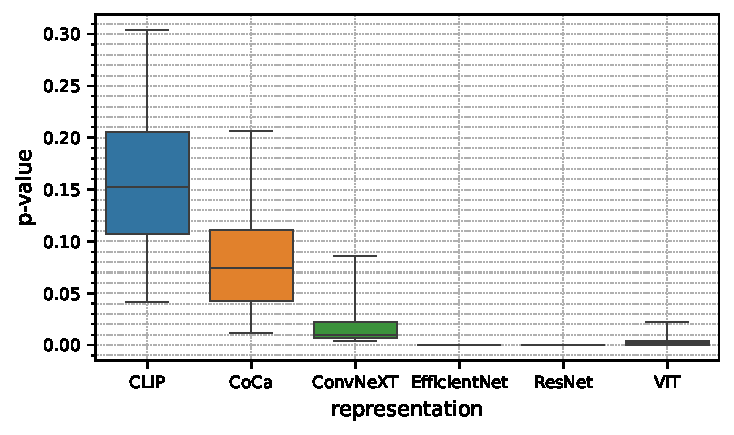
\includegraphics[width=\textwidth]{images/real-characteristics/image/properties-ImageNet-pval(representation,representation)-representation_CLIP,CoCa,ConvNeXT,EfficientNet,ResNet,ViT-class_0,999-data_ID-train.pdf}
        \label{fig:image-pvalue}
    \end{subfigure}
    \begin{subfigure}[b]{0.495\textwidth}
        \centering
        \caption{\small Kurtosis of features}
        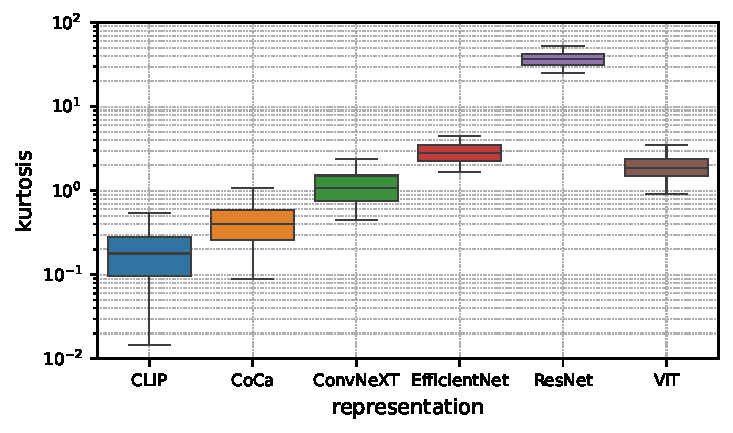
\includegraphics[width=\textwidth]{images/real-characteristics/image/properties-ImageNet-kurt(representation,representation)-representation_CLIP,CoCa,ConvNeXT,EfficientNet,ResNet,ViT-class_0,999-data_ID-train.pdf}
        \label{fig:image-curtosis}
    \end{subfigure}
    \hfill
    \begin{subfigure}[b]{0.495\textwidth}
        \centering
        \caption{\small Skewness of features}
        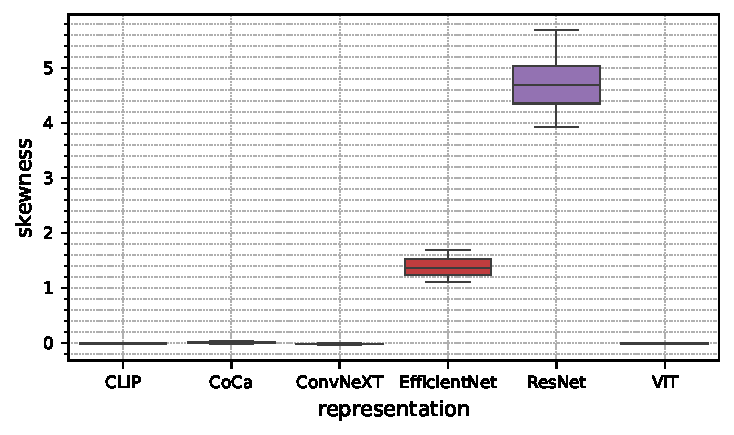
\includegraphics[width=\textwidth]{images/real-characteristics/image/properties-ImageNet-skew(representation,representation)-representation_CLIP,CoCa,ConvNeXT,EfficientNet,ResNet,ViT-class_0,999-data_ID-train.pdf}
        \label{fig:image-skewness}
    \end{subfigure}
    \caption{Properties of feature vectors corresponding to ImageNet classes obtained for 6~different representations algorithms (CLIP, CoCa, ConvNeXT, EfficientNet, ResNet~and~ViT). The same image data can be expressed as a~completely different feature~vector, depending on the chosen representation.}
    \label{fig:characteristics-image}
\end{figure}

\begin{figure}[t]
    % StreamLit settings: width=5, height=3
    \centering
    \begin{subfigure}[b]{0.495\textwidth}
        \centering
        \caption{\small Correlation of features}
        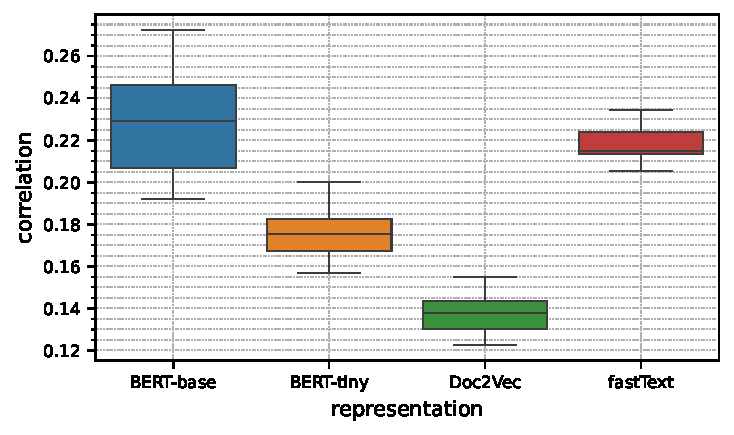
\includegraphics[width=\textwidth]{images/real-characteristics/text-20newsgroups/properties-20newsgroups-abscorr(representation,representation)-representation_BERT-base,BERT-tiny,Doc2Vec,fastText-class_0,16-data_ID-train.pdf}
        \label{fig:text-20newsgroups-abscorr}
    \end{subfigure}
    \hfill
    \begin{subfigure}[b]{0.495\textwidth}
        \centering
        \caption{\small Variance of features}
        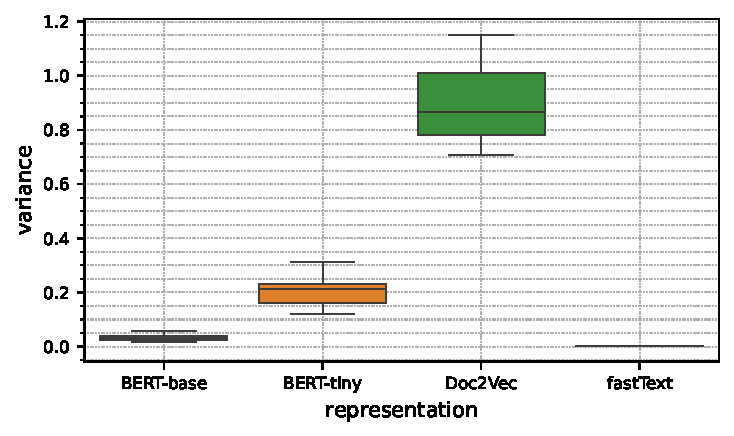
\includegraphics[width=\textwidth]{images/real-characteristics/text-20newsgroups/properties-20newsgroups-var(representation,representation)-representation_BERT-base,BERT-tiny,Doc2Vec,fastText-class_0,16-data_ID-train.pdf}
        \label{fig:text-20newsgroups-var}
    \end{subfigure}
    \begin{subfigure}[b]{0.495\textwidth}
        \centering
        \caption{\small Number of outliers per feature}
        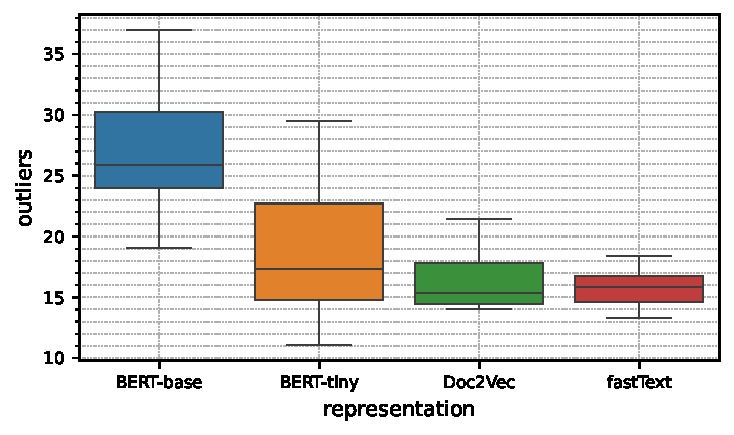
\includegraphics[width=\textwidth]{images/real-characteristics/text-20newsgroups/properties-20newsgroups-noutliers(representation,representation)-representation_BERT-base,BERT-tiny,Doc2Vec,fastText-class_0,16-data_ID-train.pdf}
        \label{fig:text-20newsgroups-outliers}
    \end{subfigure}
    \hfill
    \begin{subfigure}[b]{0.495\textwidth}
        \centering
        \caption{\small Test of features normality}
        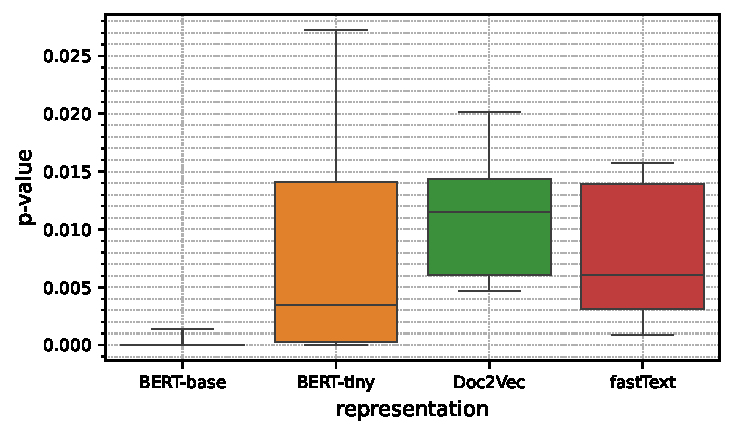
\includegraphics[width=\textwidth]{images/real-characteristics/text-20newsgroups/properties-20newsgroups-pval(representation,representation)-representation_BERT-base,BERT-tiny,Doc2Vec,fastText-class_0,16-data_ID-train.pdf}
        \label{fig:text-20newsgroups-pvalue}
    \end{subfigure}
    \begin{subfigure}[b]{0.495\textwidth}
        \centering
        \caption{\small Kurtosis of features}
        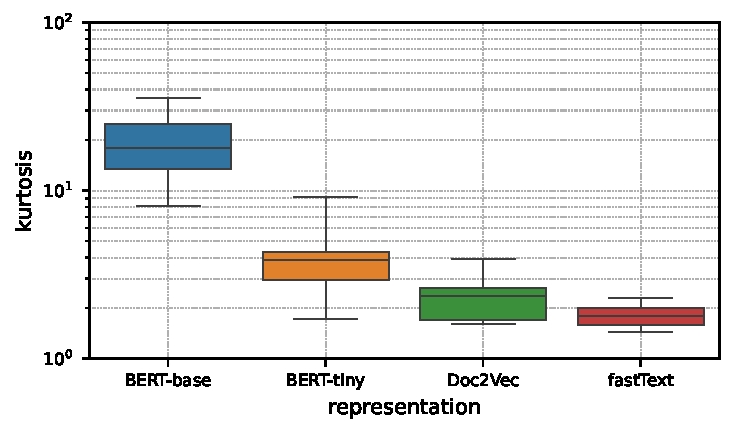
\includegraphics[width=\textwidth]{images/real-characteristics/text-20newsgroups/properties-20newsgroups-kurt(representation,representation)-representation_BERT-base,BERT-tiny,Doc2Vec,fastText-class_0,16-data_ID-train.pdf}
        \label{fig:text-20newsgroups-curtosis}
    \end{subfigure}
    \hfill
    \begin{subfigure}[b]{0.495\textwidth}
        \centering
        \caption{\small Skewness of features}
        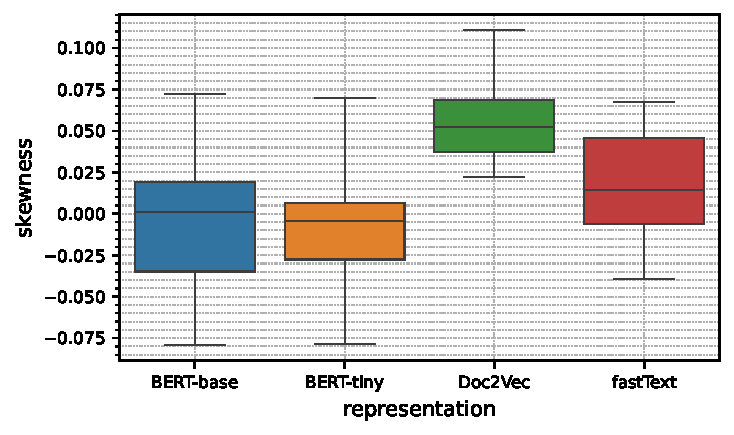
\includegraphics[width=\textwidth]{images/real-characteristics/text-20newsgroups/properties-20newsgroups-skew(representation,representation)-representation_BERT-base,BERT-tiny,Doc2Vec,fastText-class_0,16-data_ID-train.pdf}
        \label{fig:text-20newsgroups-skewness}
    \end{subfigure}
    \caption{Properties of feature vectors corresponding to 20newsgroups classes obtained for different representations algorithms (BERT, Doc2Vec and fastText). Analysis for TF-IDF was omitted due to the size of feature vectors.}
    \label{fig:characteristics-text-20newsgroups}
\end{figure}

\begin{figure}[t]
    % StreamLit settings: width=5, height=3
    \centering
    \begin{subfigure}[b]{0.495\textwidth}
        \centering
        \caption{\small Correlation of features}
        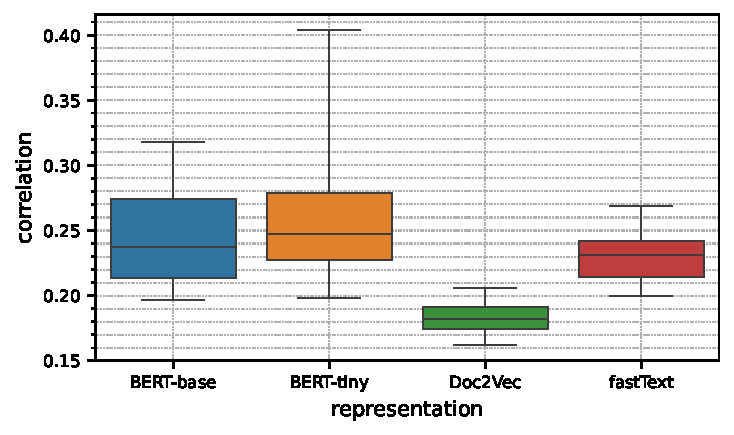
\includegraphics[width=\textwidth]{images/real-characteristics/text-banking77/properties-banking77-abscorr(representation,representation)-representation_BERT-base,BERT-tiny,Doc2Vec,fastText-class_0,61-data_ID-train.pdf}
        \label{fig:text-banking77-abscorr}
    \end{subfigure}
    \hfill
    \begin{subfigure}[b]{0.495\textwidth}
        \centering
        \caption{\small Variance of features}
        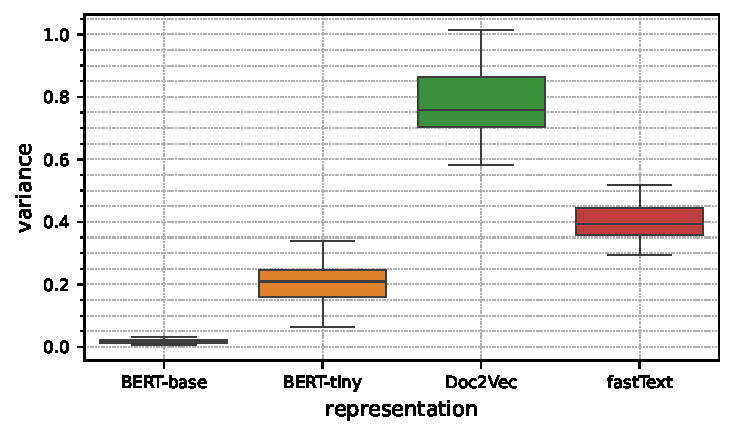
\includegraphics[width=\textwidth]{images/real-characteristics/text-banking77/properties-banking77-var(representation,representation)-representation_BERT-base,BERT-tiny,Doc2Vec,fastText-class_0,61-data_ID-train.pdf}
        \label{fig:text-banking77-var}
    \end{subfigure}
    \begin{subfigure}[b]{0.495\textwidth}
        \centering
        \caption{\small Number of outliers per feature}
        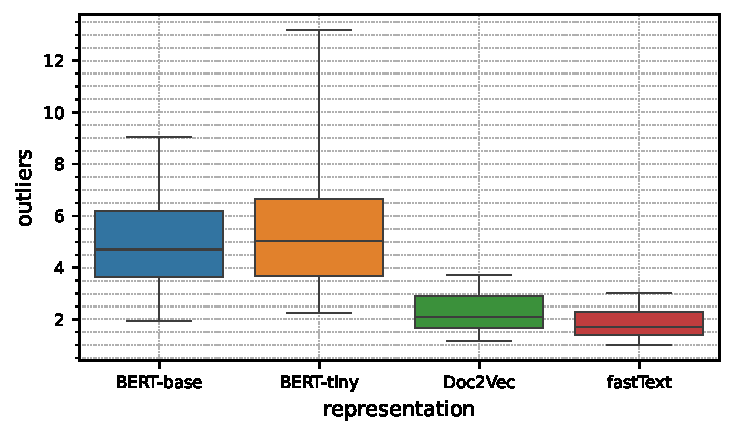
\includegraphics[width=\textwidth]{images/real-characteristics/text-banking77/properties-banking77-noutliers(representation,representation)-representation_BERT-base,BERT-tiny,Doc2Vec,fastText-class_0,61-data_ID-train.pdf}
        \label{fig:text-banking77-outliers}
    \end{subfigure}
    \hfill
    \begin{subfigure}[b]{0.495\textwidth}
        \centering
        \caption{\small Test of features normality}
        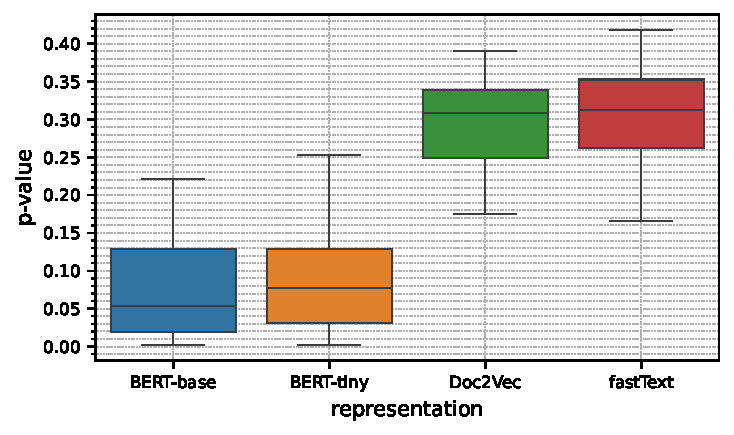
\includegraphics[width=\textwidth]{images/real-characteristics/text-banking77/properties-banking77-pval(representation,representation)-representation_BERT-base,BERT-tiny,Doc2Vec,fastText-class_0,61-data_ID-train.pdf}
        \label{fig:text-banking77-pvalue}
    \end{subfigure}
    \begin{subfigure}[b]{0.495\textwidth}
        \centering
        \caption{\small Kurtosis of features}
        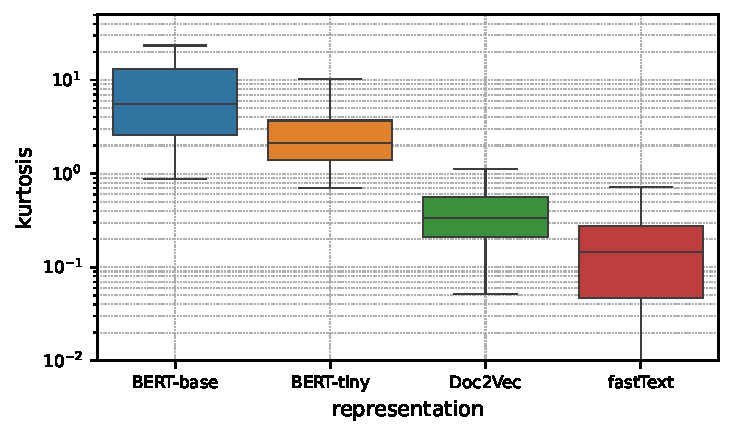
\includegraphics[width=\textwidth]{images/real-characteristics/text-banking77/properties-banking77-kurt(representation,representation)-representation_BERT-base,BERT-tiny,Doc2Vec,fastText-class_0,61-data_ID-train.pdf}
        \label{fig:text-banking77-curtosis}
    \end{subfigure}
    \hfill
    \begin{subfigure}[b]{0.495\textwidth}
        \centering
        \caption{\small Skewness of features}
        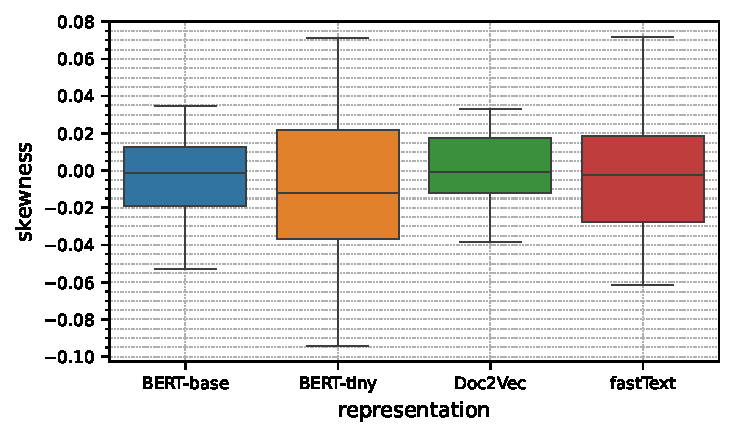
\includegraphics[width=\textwidth]{images/real-characteristics/text-banking77/properties-banking77-skew(representation,representation)-representation_BERT-base,BERT-tiny,Doc2Vec,fastText-class_0,61-data_ID-train.pdf}
        \label{fig:text-banking77-skewness}
    \end{subfigure}
    \caption{Properties of feature vectors corresponding to banking77 classes obtained for different representations algorithms (BERT, Doc2Vec and fastText). Analysis~for~TF-IDF was omitted due to the size of feature vectors.}
    \label{fig:characteristics-text-banking77}
\end{figure}

\cleardoublepage{}
